%%%%%%%%%%%%%%%%%%%%%%%%%%%%%%%%%%%%%%%%%%
%%%                                    %%%
%%% (c) Vojtěch Kopal, 2011            %%%
%%%                                    %%%
%%%%%%%%%%%%%%%%%%%%%%%%%%%%%%%%%%%%%%%%%%


%\documentclass[12pt,notitlepage]{report}
%\pagestyle{headings}
\pagestyle{plain}

\documentclass[12pt,a4paper]{report}
\setlength\textwidth{145mm}
\setlength\textheight{247mm}
\setlength\oddsidemargin{15mm}
\setlength\evensidemargin{15mm}
\setlength\topmargin{0mm}
\setlength\headsep{0mm}
\setlength\headheight{0mm}
% \openright zařídí, aby následující text začínal na pravé straně knihy
\let\openright=\clearpage

%\frenchspacing % aktivuje použití některých českých typografických pravidel

\usepackage[utf8]{inputenc} % nastavuje použité kódování, uživatelé Windows zamění latin2 za cp1250
\usepackage[T1]{fontenc}
\usepackage{a4wide} % nastavuje standardní evropský formát stránek A4
%\usepackage{index} % nutno použít v případě tvorby rejstříku balíčkem makeindex
%\usepackage{fancybox} % umožňuje pokročilé rámečkování :-)
\usepackage{graphicx} % nezbytné pro standardní vkládání obrázků do dokumentu
\usepackage{enumerate}
\usepackage{listings}
\usepackage[left=4cm]{geometry} % nastavení dané velikosti okrajů
\usepackage[dvips]{color}
\usepackage{subfigure}
\usepackage{amssymb,amsmath}

%\newindex{default}{idx}{ind}{Rejstřík} % zavádí rejstřík v případě použití balíku index
\usepackage[ps2pdf,unicode]{hyperref}   % Musí být za všemi ostatními balíčky
\hypersetup{pdftitle=Komunikace a paměť pro plausibilní agenty}
\hypersetup{pdfauthor=Vojtěch Kopal}

\newtheorem{definition}{Definition}
\newtheorem{example}{Example}

\title{Komunikace a paměť pro plausibilní agenty}   % tyto dvě položky jsou zde v podstatě formálně, ve skutečnosti nejsou nikde 
\author{Vojtěch Kopal} % dále v dokumentu použity

%\date{}

\begin{document}

%\csprimeson % zapne jednoduché psaní českých uvozovek pomocí klasických znaků, ale potom pozor 
             % na originální apostrofy, které budou chybně interpretovány!!!

%%% Následuje první, úvodní, strana bakalářské práce. Jednotlivé položky nahraďte dle vlastních
%%% údajů. Změnit podle konkrétní délky jednotlivých položek můžete i zalomení řádků.
\begin{titlepage}
\begin{center}
\ \\

\vspace{15mm}

\large
Charles University in Prague\\
Faculty of Mathematics and Physics\\

\vspace{5mm}
   
{\Large\bf BACHELOR THESIS}

\vspace{10mm}

%%% Aby vložní loga vše správně fungovalo, je třeba mít soubor logo.eps nahraný v pracovním adresáři,
%%% tj. v adresáři, kde se nachází překládaný zdrojový soubor. Soubor logo.eps je možné získat např.
%%% na adrese: http://www.mff.cuni.cz/fakulta/symboly/logo.eps

\includegraphics[scale=0.3]{logo.eps} 

\vspace{15mm}

%\normalsize
{\Large Vojtěch Kopal}\\ % doplňte vaše jméno
\vspace{5mm}
{\Large\bf Komunikace a pamě\v{t} pro plausibilní agenty}\\ % doplňte název práce       
\vspace{3mm}
{\Large\bf Communication and memory in plausible agents}\\ % doplňte název práce     
\vspace{5mm}
{\Large Department of Theoretical Computer Science and Mathematical Logic}\\
\end{center}
\vspace{10mm}

\large
\noindent Supervisor: Mgr. Ondřej Sýkora
\vspace{1mm} 

\noindent Study programme: Computer Science

\noindent Specialization: General Computer Science

\vspace{10mm}

\begin{center}
2011
\end{center}

\end{titlepage} % zde končí úvodní strana

\normalsize % nastavení normální velikosti fontu
\setcounter{page}{2} % nastavení číslování stránek
\ \vspace{10mm} 

\noindent In the first place I would like to thank my supervisor, Mgr. Ondřej Sýkora, for providing guidance in my work and allowing me finish it. I also want to thank my friends MSc M. Bernát, Bc. J. Helmich and Bc. M. Mráz for their time and proofreading my work. Finally, I want to thank everyone who stayed with me till this end. % doplňte vlastní text

\newpage

\vglue 0pt plus 1fill

\vspace{\fill} % nastavuje dynamické umístění následujícího textu do spodní části stránky
\noindent I declare that I carried out this bachelor thesis independently, and only with the cited 
sources, literature and other professional sources. 

\noindent I understand that my work relates to the rights and obligations under the Act No. 
121/2000 Coll., the Copyright Act, as amended, in particular the fact that the Charles 
University in Prague has the right to conclude a license agreement on the use of this 
work as a school work pursuant to Section 60 paragraph 1 of the Copyright Act. 

\bigskip
\noindent In Prague date 5th August 2011\hspace{\fill}Vojtěch Kopal\\ % doplňte patřičné datum, jméno a příjmení

%%%   Výtisk pak na tomto míste nezapomeňte PODEPSAT!
%%%                                         *********

\setcounter{tocdepth}{1}
\tableofcontents % vkládá automaticky generovaný obsah dokumentu

\newpage % přechod na novou stránku

%%% Následuje strana s abstrakty. Doplňte vlastní údaje.
\noindent
Název práce: Komunikace a pamě\v{t} pro plausibilní agenty\\
Autor: Vojtěch Kopal\\
Katedra (ústav): Katedra teoretické informatiky a matematické logiky\\
Vedoucí bakalářské práce: Mgr. Ondřej Sýkora\\
e-mail vedoucího: mail@ondrejsykora.com\\

\noindent Abstrakt:  V předložené práci jsme se zaměřili na porovnávání různých implementací pamětí pro plausibilní agenty v multi-agentním prostředí. Vytvořil jsem simulaci, ve které se snaží jednotliví agenti naplňovat svou potřebu jíst. Aby uspěli musí se naučit, kde jsou zdroje potravy, k čemuž jim slouží implementovaná prostorová paměť a schopnost komunikovat mezi sebou. Agenti jsou posléze hodnoceni podle úrovně hladu v průběhu simulace. \\

\noindent Klíčová slova: plausibilní agenti, prostorová paměť, growing neural gas, komunikace

\vspace{10mm}

\noindent
Title: Communication and memory in plausible agents\\
Author: Vojtěch Kopal\\
Department: Department of Theoretical Computer Science and Mathematical Logic\\
Supervisor: Mgr. Ondřej Sýkora\\
Supervisor's e-mail address: mail@ondrejsykora.com\\

\noindent Abstract: In the present work we have focused on comparation of different implementation of memory for plausible agents in multi-agent environment. I have created a simulation whereby the agent are strangling to fulfill their need to eat. To succeed they have to learn the locations of food resources using the implemented spatial memory and an ability to communicate with each other. Later the agents are evaluated according to the level of hunger throughout the simulation.\\

\noindent Keywords: plausible agents, spatial memory, growing neural gas, communication

\newpage

%%% Následuje text bakalářské práce členěný do kapitol, které se číslují, označí názvy a graficky oddělí.
%%% Nedoporučuje se používat víc než dvě úrovně číslování kapitol, viz příklad níže.

\chapter{Introduction}

In a modern society the amount of information is far behind what one can remember or even process. If we understand that, we realize how important it is to be able to delegate the thinking amongs group. The decision making in groups and teams is a topic covered by several papers. [citation required] Supposing we have limited capacity of memory, we have to distribute the knowledge amongst people around us and communicate with each other so as to gather facts which we currently need to make the decision. 

Our decisions are either consciously or subliminaly based on our needs or drives - former term might be rather connected with human behavior, latter term is used for plausible agents. As in microeconomics we can use an utility as a measure of relative satisfaction \cite{Varian:micro} and see how one manages fulfilling their needs. While attaining the goals we use a knowledge which we store in our memory and which we update regularly. With infinite memory we wouldn’t have any problems to store all information and use it when required; however, we don’t have such memory - our memory is limited. 

What I mean by saying “not to have enough space in our memory” is one is not able to remember everything. Certain pieces of information are fading away as time goes or as one is learning new facts. I want to observer if and how an intensive communication can substitute insufficient memory space with the condition of constant level of utility.

Is it obvious that adding the ability of communication improves the agents'chances to survive in the environment.

I want to observer the relation between amount of communication and used spatial resource-bounded memory. 

This thesis consists of [N] parts. First, I will introduce the topic of agent and possible memory implementations based on concrete examples (Chapter 2). Then I will explain what algorithms, such as growing neural gas, I am going to use in the program (Chapter 3). In \emph{Chapter 4} there is a description of the simulation, agents, their memory and the communication.

\chapter{Related work}

I will use this chapter as an insight into the world of agents and spatial memory. I hope that you will not be disappointed, since there is no 007 in following lines.

\section{Agents}

There are several ways how to explain what or who the agent is. Apart from systems of agents used in philosophy or sociology, we can see a first modern use of agency and agents in economy where economists have substited the human with a simpler agent. They intended to simplify their economic models to be able to actually simulate something. Buyers and sellers are typical examples of agents used in simplified market model in microeconomics (see []). In this context agents are entities in the model which can act based on situation in the model.

For area of artificial intelligence we can use the definition of an agent which can be found in \cite{russel2003ai}. It cannot be more simple:

\begin{definition}{\bf Agent} is just something that acts.
\end{definition} 

Of course it is as general as it could be and for my purposes it is too simple, so I will use another definition which meets better the context of my work.

\begin{definition}{\bf Agent} is something that senses the environment and affects it using its actuators.
\end{definition} 

Having that defined we continue to specific kinds of agent. In this thesis I use several slightly varying terms about agents: {\emph rational, autonomous, plausible and believable}. 

A rational agent refers back to economics where we can find a definition of rational behaviour. Even though it is rather a hypothetical model, as people are usually irrational in their decisions from the economics perspective, their is yet nice definition whereby a rational agent acts as if balancing costs against benefits to arrive at action that maximizes personal advantage (Milton Friedman (1953), Essays in Positive Economics). So simply he does what is or perhaps might be best for him based on his current knowledge of the world.
 
On the other hand, the rational behaviour might be understood in a completely different way. Plausible agents are such agents, where the basic approach is to implement human-like internal processes. One of the well-known example is neural networks, although they are usually used in quite simplified way. Since it is really difficult to implement completely plausible agent, one can see research teams focusing on a specific part of the complex human being. 

Autonomous agents are those agents which are capable of accomplishing useful tasks or are effective problem solvers \cite{Loyall:believableagents}. A

Believable agents are personality-rich autonomous agents with the powerful properties of characters from the arts \cite{Loyall:believableagents}. Now there is just the autonomous agent left. An autonomous agent should be able to accomplish useful task or be an effective problem solver. I would like to add one more term which is going to fit the agents I use. 

Belief-Desire-Intention (BDI) agency model implements the three parts agent's belief, desire and intention and use them when comes to reasoning. A BDI agent is particular part of bounded rational agent who use those three parts to separatly prepare plans which are later executed. What a BDI distinguishes from a simple reactive agent is a reactive agent creates immediate decisions based on current state of environment and inputs of his sensors. On the other hand, a BDI agent uses the three parts:

\begin{itemize}
\item {\bf belief} represents the agent's informational state, for example sensory inputs and information in his memory,
\item {\bf desire} is the agent's motivational state, what he needs to approach, for example he is hungry and he needs to find appropriate food,
\item {\bf intention}, on the other hand, is his immediate decision how he attaing the goal he desires, in other words it is execution of plan, for example next move.
\end{itemize}

\section{Spatial resource-bounded memory}

A memory is something what changes a reactive agent into an agent with ability to learn. It can be used for learing consequances of agent's acts, conditional dependencies in the agent's world (citation for bayesian networks), or spatial information about the environment. The latter one is a kind of memory I used for agents in my simulation. 

A spatial memory is used when agent needs to navigate in usually two or three dimensional space. In short it is a component of an agent which says him where to go when he needs or want to do something. There are several different approaches and a couple of examples are going to be covered in this section. I am going to introduce several existing implementations of spatial memory. Mainly I will focus on if and how they have dealt with bounded resources - either due to implementation restrictions, or when approaching plausibility in their models. 

\subsection{Resource-bounded reasoning}

Rational agents cannot be expected to be able to compute a load of data in a constant time or in a time in which the environment doesn't change much. That is why we have to take into account bounded resources when simulating plausible or rather real agents. What we want to avoid here is the computation of plan takes a long period of time during which the environment changes significantly. As they have mentioned in \cite{Bratman:practicalreasoning}, we could separate plan computation from execting the plan, whereby the plan is prepaired over several executions. In that case we need either to be able to perfectly predict the future, or base our plan on data which does not change at all or is frozen for the given period of time.

\subsection{Short-term and long-term memories}

Generally, when I talk about remembering something I should mention two terms: a long-term memory (LTM) and a short-term memory (STM). Both of which describes a capacity for holding certain amount of information in mind. Apart from the varying amount, the memories differ in availability of such information and a period of time the memories last.       

Short-term memory (...)

Long-term memory (...)

\subsection{Computational memory architectures}

Computational memory architectures for autobiographic agents interacting in complex virtual environment suggested by Ho in \cite{Ho:memoryarchitectures}. works with both short-term and long-term autobigraphic memory, where they have observed agent’s ability to survive comparing to purely reactive agency model. Moreover, they researched whether the narrative communication amongst agents somehow positively influence those agents. They have separately experimented with three types of agents: purely reactive (PR), short-term memory (STM) and long-term memory (LTM). Purely reactive agent walks randomly around the environment avoiding obstacles and searching for resource objects to fulfill his needs. What a pure reactivity means is the agent moves randomly until an event occurred such as a collision with obstacle or a resource object detection.

STM agents in \cite{Ho:memoryarchitectures} further extend the model of purely reactive agents and add a Track-back memory system in addition to the reactive behaviour. Each time an agent deals with an event (e.g. collision, or resource object) he puts such information into his memory. They refer to this as an event-based memory entry making mode. Those events are kept in a linear list of a finite size, whereby the oldest events are cut off. The memory is used when an internal variable is over threshold. That is the moment when agent searches in his memory for an information about relevant resource object. If he succeeded, he retrospectively undoes all memorized states leading to the relevant one. So, what they actually store in memory is an agent’s current state: where he was and what he perceived. While attaining imperfection in retrieving information from short-term memory, they introduced noise distortion using Gaussians.

Long-term memory model is mostly based on psychological autobiographic memory models. There are three parts that are involved in the reasoning process: Event specific knowledge (ESK), Event reconstruction process (ER) and Event filtering and ranking process.

\subsection{Inspirations for my work}



%Former one is responsible for storing event history in a similar way as the event-based memory entry making mode. A stored record contains what objects and environment were around the agent, and values of internal variables. Those values are used as various kinds of keys: match key, search key, and conditions, where search key means the resource which can be obtained if conditions hold in the area specified by match key. 

%As in PR model, the ER is fired when there is an internal variable which is below the threshold. At that moment, the agent goes through ESK and search for relevant record. Such a record has to have an equivalent search key to the type of the low internal variable. It is possible for ER to return more than one relevant record. A reconstruction of appropriate number of events leading to the state described by the record is one important part of the following EFR processes. To reach the desired state we can either Redo the memorized steps which had led to the state, or we can Undo the steps which followed, that means to go through them in a reverse order. 

%Finally, I have mentioned that ER can resolve more than one record, which happens after longer period of time when an agent luckily survived in the environment and, subsequently, managed to fill his ESK with sufficient amount of information. At that moment, there has to be a filtering process, which chooses the best record to be proceeded. EFR processes first filter out records that do not match current state of the environment and then order the rest according to how much they better off the agent’s internal variables.

%As an addition to LTM agents they introduced communicative agents with long-term memory, which are able to share their knowledge among each other. First, they extended the structure of ESK, so as to keep a variable about who is the source of the records. Then they defined a communication protocol between two agents, whereby one agent has a role of story-teller and the other one is a listener. The listener ask the story-teller about a object resource and story-teller returns a best story generated by the same process he normally during his reasoning process.

%During experiments they measured the lifespan of agents, and also observed levels of internal variables for sample agents representing one of each suggested models. It was expected that more complex memory structures led to better results and such assumptions were proved correct. A combination of RTM and LTM was clearly the best model and agents with this model where able to live with the least drops in their internal variables and generally their lives were rather stable comparing to others.

%[“What is interesting in it for me”]

%The suggested RTM and LTM models of agents are more than interesting to be implemented in my simulation. There has to be a couple of minor changes, though, as I am working with a simpler environment comparing to the one used in the work described above. The changes will influence the structure of memory records in both RTM and LTM. Also the communication protocol will be different and I am going to introduce it later in this thesis.



\chapter{Used methods and algorithms}

In previous chapter I have introduced you to several kinds of agents, how they can be used and also what a spatial memory is. I have briefly prepaired you for the next chapters, where I will explain my contribution to this area. This chapter is going to cover the used algorithms and computational methods I have studied and implemented in my work. 

The first subsection disserts on the implementations of agents' memory and in detail describes fundamental parts. Both the Growing Neural Gas and the Quad..blah are used as memory storages to handle spatial information about the environment with bounded resources.

\section{Growing Neural Gas}   
\label{usedalgo:gng}

\subsection{Topology learning}

Processing an enormous spatial data about an environment is computationaly demanding when for example we want to navigate in that environment. A topology learning or recognition can help us to create a representation such as topological map which can be viewed as a graph and which makes reasoning in that environment much easier. Rather complex understanding of topology in an indoor space using Bayesian programming has been shown in \cite{Tapus:topologylearning}. It goes much farther than I need to. 

Based on competitive Hebbian learning (CHL) method \cite{Martinetz:chl} and Neural Gas (NG) \cite{Martinetz:ng} Bern Fritzke suggested earlier mentioned Growing Neural Gas \cite{Fritzke:gng}, an unsupervised learning method for finding a topological structure which reflects the topology of the data distribution. Although the combination of both CHL and NG is an effective method for topology learning, there are some flaws in practical application as it requires an initial setup of number of nodes/centers that are used. This fact prevents the method from adequately describing the topology, when a different number of nodes would work better.

As Fritzke described the algorithm uses a set of nodes and edges that connects the nodes. A simplified describtion of algorithm from \cite{Fritzke:gng} in context of two-dimensional space follows:

\begin{enumerate}
\item Add two nodes at random position onto canvas
\item Generate input signal based on the data distribution (its probability density)
\item Find the nearest node $n_1$ and second nearest node $n_2$ to the signal
\item Increment the age of all edges leading from node $n_2$
\item Add the squared distance between the input signal and the nearest unit in
input space to a local counter variable $\Delta error(n_{1})$
\item Moved node $n_1$ and its topological neighbors towards the signal (according to parametres $epsilon_{winner}$ and $epsilon_{neighbour}$)
\item Remove all edges with an age larger than $a_{max}$
\item Generate new nodes (see \cite{Fritzke:gng}) using variable $alpha$
\item Decrease all error variables by multiplying them with a constant $beta$
\item Go to 1.
\end{enumerate}

For the purpose of this work I want to use this algorithm to learn a topology of data which dynamically changes through the time. We have to setup the variables for this agorithm $alpha$, $beta$, $epsilon_{winner}$, $epsilon_{neighbour}$ and maximal number of nodes. In following subsection I am going to introduce you to the experimenting with this algorithm.

\subsection{Experiments on dynamic data}

As I have mentioned previously I had to setup the variables so as to be able to use Growing Neural Gas method properly. To attain this goal I have made a Java programm which tests various combinations of variables' values and finds the best one. It has sequently run the algorithm for a given number of steps and measured the \emph{score} (see \ref{usedalgo:scoremethod}).

\begin{figure}
\begin{lstlisting}[language=Pascal]
procedure Score()
  (px, py, pvar) <- GetProbableGauss()
  (rx, ry, rvar) <- GetRealGauss()
  
  sqDistance <- (px - rx)*(px - rx) + (py - ry)*(py - ry)
  sqSize <- (pvar + rvar)*(pvar + rvar)
  
  score <- sqDistance / sqSize
  
  return score
end
\end{lstlisting}       
\caption{The \emph{SCORE} method}
\label{usedalgo:scoremethod}
\end{figure}
       
\begin{figure}      
\begin{center}
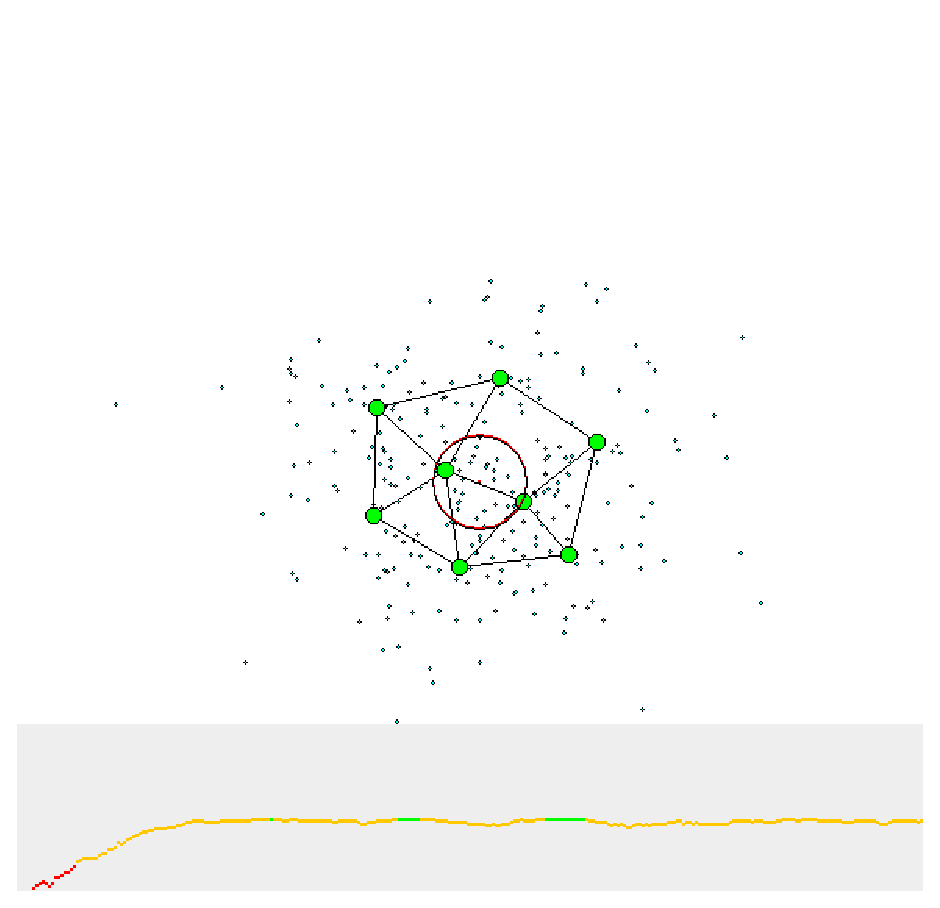
\includegraphics[scale=0.75]{images/gng/experimental_setup.eps}    
\caption{Screenshot showing the process of searching optimal variable values. The visualization has been made for testing purposes in the first place, but it nicely shows what had been lately paralelly computed. The bottom part of the picture shows the SCORE value throughout the simulation. {\emph (Red color means $SCORE > 0.05$, orange is $SCORE > 0.001$ and green is $SCORE <= 0.001$)} }
\end{center}                          
\label{usedalgo:gngexperimentscreen}
\end{figure}

\begin{figure}          
\begin{itemize}
\item $alpha \in \{0.0, 0.2, 0.4, 0.5, 0.6, 0.8, 1.0\}$
\item $beta \in \{0.0, 0.00001, 0.00005, 0.0001, 0.001, 0.005, 0.01, 0.5, 0.1, 0.5, 1.0\}$
\item $epsilon_{winner} \in \{0.0, 0.001, 0.005, 0.01, 0.1, 0.2, 0.5, 1.0\}$
\item $epsilon_{neighbour} \in \{0.0, 0.0001, 0.0006, 0.001, 0.005, 0.05, 0.1, 0.2\}$
\item $maxNodes \in \{4, 8, 16, 32\}$
\end{itemize}
\caption{Domains of variables for the experimental learning of best values.}
\label{usedalgo:gngexperimentdomains}
\end{figure}

A total number of possible combinations is equal to 19712. For each such a combination I have run 10000 steps of GNG learning sequence and measured the average score. Each sequence took aproximately 108 seconds and all the experiment was computed paralelly using 30 threads.

The best results which were avarage $SCORE < 10^{-11}$ is shown in a table \ref{usedalgo:gngexperimentresults}.

\begin{table}
\begin{center}
\begin{tabular}{ccccc|c}

$alpha$ & $beta$ & $epsilon_{winner}$ & $epsilon_{neighbour}$ & $numNodes$ & $SCORE$ \\
\hline
0.0 & 1.0 & 0.0050 & 0.0 & 16 & $3.8*10^{-12}$ \\
0.5 & 0.0 & 0.01 & 1.0E-4 & 8 & $5.1*10^{-12}$ \\   
0.5 & 0.0010 & 0.1 & 0.0010 & 8 & $8.8*10^{-12}$ \\ 
0.5 & 1.0 & 0.0 & 1.0E-4 & 8 & $3.1*10^{-12}$ \\     
0.8 & 1.0E-5 & 0.0010 & 1.0E-4 & 32 & $7.4*10^{-12}$ \\
0.8 & 1.0E-5 & 0.0050 & 6.0E-4 & 8 & $4.3*10^{-12}$ \\

\end{tabular}      
\caption{\label{usedalgo:gngexperimentresults}Variable values with best average SCOREs}
\end{center}
\end{table}

\section{Grid}
\label{sec:grid}

The idea for this data structure representing resource-bounded memory is based on \cite{Brom:placeandobjects}. What differs in my work from their observed environment is agents in my simulation act in a homogeneous space which cannot be differentiated in a way the mentioned simulation does. To solve this issue I have simply differentiated the environment into grid 4x4, where each cell works as the place in \cite{Brom:placeandobjects}. 

Each cell is given two variables {\emph positive} and {\emph negative} both of which are set to zero and increased throughout the simulation. When an agent sees at least half of that area determined by the cell, if he sees any food, he increase the {\emph positive} variable. If the agent search for food and he cannot see any, he increase the {\emph negative} variable.

When the grid is later asked whether there is food at specific cell, it answers according to this method with parametr $\alpha$ to be found:

\begin{equation} ANSWER = \alpha\times positive - negative 
\end{equation}
 
Similary I will use this structure to keep spatial information about the environment in the simulation.

\chapter{Simulation and used memory architectures}

In this chapter I will describe the simulation, environment and agent's reasoning and communication how it is used in later experiments. 

\section{Simulation}

The {\bf simulation} is consists of a set of agents, a set of generators and a set of pieces of food. According to given settings it sequently processes a number of steps, each of which invokes an agents' life step and eventually generating new food.

It can also contains a couple of monitors which observe the environment or agents.

\section{Environment}

The environemt si a two-dimensional space which contains agents and food. Agents can move around and eat the food which is randomly distributed using the food generators. 

\section{Agent}                                                      

As I mentioned previously an agent is an entity in the environment which moves and interact with the world around. The interaction is done through eating food which is a part of the environment and through communication with other agents. The latter one actually changes agents' believes about the environment.

Agent has his needs which influences his desicions as fulfilling his needs keeps him alive. When his internal variables of needs is higher than    

There are four types of agents each of which is different in the way they decide about next step. If one is hungry and sees a food (i.e. there is a piece of food in the sight distance) then they choose to go after this food. If there is no desired food around they go searching for it and that is when differs the agents' actions.

\begin{itemize}
\item \emph{random agent} moves randomly around the environment,
\item \emph{pure reactive agent} sees the whole environment, i.e. they always sees a desired piece of food, 
\item \emph{grid agent} implements a memory based on clustering the space into a grid,
\item \emph{GNG agent} implements a memory based on growing neural gas.
\end{itemize}

\section{Communication}

Apart from what agent sees, there is another way how the agents gather information about the environment. They communicate. It is quite simple way of sharing information. When suggesting an implementation for communication I had to create a unified protocol which could have been used throughout types of agents. Thereby I have tried to have this communication protocol as simple as possible.

Moreover, although all agents have a kind of knowledge about the environment they are not able to answer easily, when they are asked about a specific food location. Since the food appears in environment according to given normal distribution, it is not clear what should be an answer for such question. A couple of possible kinds of answers follows. 

First and the most simple answer might be saying exact X,Y coordinates of the food location as it is stored in agent's mind. Additionaly, there would be a noise added to such an answer, having in mind that the answer should not be perfect and there is always a distortion and inperfection in our answers based on how a person is certain about his answer.
                                              
Another way and possibly more plausible one might be answering by a direction (an angle) with an approximate distance. What both the first suggested XY answer and this one have in common is the answers are hard to combine with the learning method used in GNG memory. GNG works with samples of data which sequently influence the neural network. Both kinds of answers could be used if agents would ask more often or the agent's answer would be a sample of points rightaway.

Having such conditions I have suggested and implemented a communication \ref{solution:decision} where the answer consists of several sample points which are generated according agent's knowledge.

\begin{figure}
  \centering                                
  \includegraphics[scale=0.7]{diagrams/solution/communication.eps}    
  \caption{Simple communication protocol}
  \label{solution:communication}
\end{figure}

\section{Decision making}

While searching for food each type of agents makes the decision where to go next. This process is either done randomly or following ones knowledge of the environment around. A simple diagram of decision making follows.

\begin{figure}
  \centering                                
  \includegraphics[scale=0.7]{diagrams/solution/decision-flowchart.eps}    
  \caption{How the agent decides what to do next}
  \label{solution:decision}
\end{figure}

The diagram \ref{solution:decision} shows how an agents decides what to do. In fact it is common for all types of agents described in this thesis, although the first step "Put known food location into memory" is ommited in case of \emph{random} and \emph{PR agents}.

\section{Memories}

There are two types of memory which should allow agents to improve their lifespan comparing to a random agent. Those are memories based on a growing neural gas and a spatial grid.       

The \emph{GNG memory} uses a self-teaching neural network which has been described in \ref{usedalgo:gng}. The neural network allows the agent to learn approximate location where the food is distributed. Each food kind is given a single neural network which tries to learn the distribution reflecting the data inputs.

The \emph{grid memory} divides the environment into a grid so as to simplify the space and restrict total size of data structure used to describe the space. 






\chapter{Implementation}

\section{Data structures}

In this section I will introduce the data structure that were used to implement each part of the simulation. 









                                    

\chapter{Experiments}

%\section{Notes}

%The fact is the more an agent actually sees the more successful he is in staying alive.

%Too much communication might lead to disorientation of an agent which is subsequently followed by agent's death.

\section{Experimental settings and methodology}

All following experiments are run using a default setup as it is described in this section. Each of the experiments is run on a quadcore \emph{Intel Core i5 with 2,4 GHz and 6 GB RAM}. 
                                                   
Environment is set to be a square matrix with \emph{64 x 64 dimension}. All agents start in the middle of the environment. There are \emph{six kinds of food} which are randomly positioned in the environment and which generate a piece of food each \emph{50 steps}.

Since an environment contains of six food kinds, an agent has six internal variables for each such food kind (see \ref{experiments:singleagent}). By default they are set to 0 and are increased by \emph{0.001 each step} in simulation. When they are equal to 1 (or higher), the agent dies.  

\begin{figure}[h!]
  \centering                                
  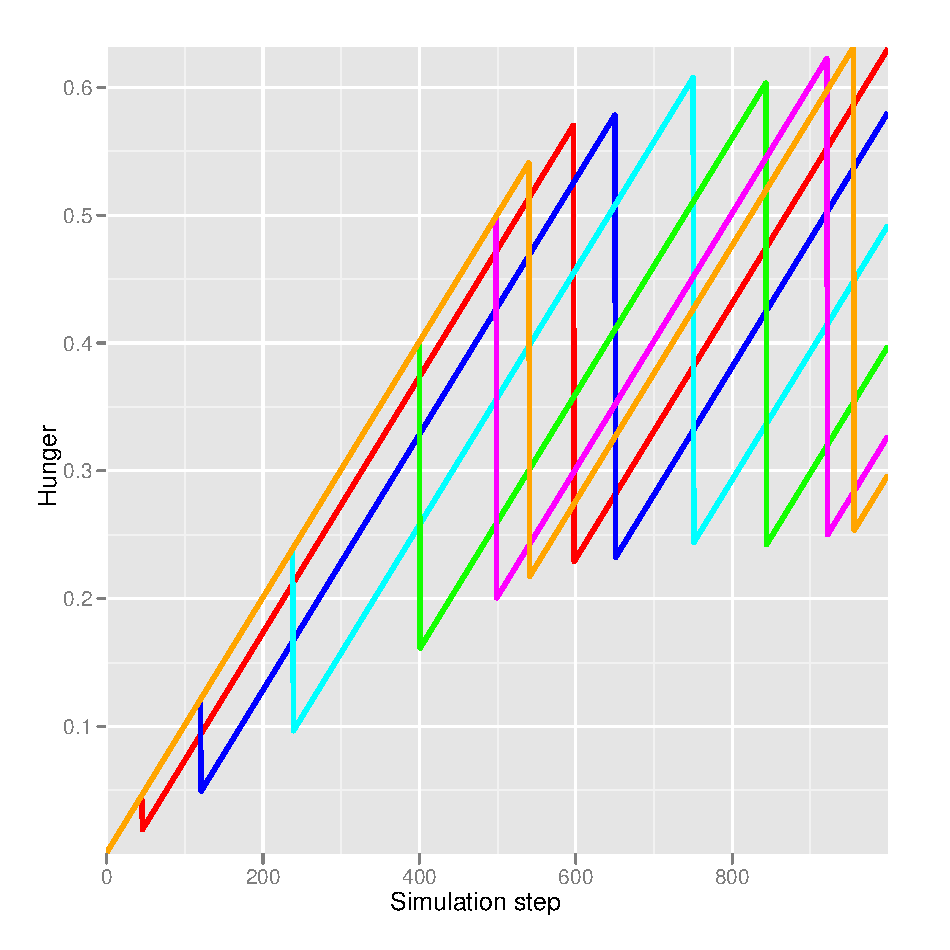
\includegraphics[scale=0.4]{diagrams/experiments/single_agent.eps}    
  \caption{An example of agent's first 1000 steps showing the needs for each kind of food.}
  \label{experiments:singleagent}
\end{figure}



\section{Homogeneus agent set comparision with communication}

In this experiment I will compare avarage life span and efficiency of groups which contains of agents with only single type of memory. Thereby you can see which of the used memory implementation works better in memory homogeneus environment.

What I assume is the \emph{random agents} are about to expire almost immediately as they had no chance to find all the food. While the \emph{PR agents} should approach their goals easily, thereby they will stay alive. Both results of \emph{GNG agent} and \emph{grid agent} are matters of the experiment and I can only expect them not to be worse than \emph{random agent} and not to be better than \emph{PR agent}.     

\clearpage

\subsection{Random agent}   

As for the random agents I assumed that they will immediately pass away without communication. And as you can see in \ref{experiments:random-silent} it happened to be true. 

On the other hand, if I allow them to communicate with each other it might happen they improve their chances. Although they will not last through the entire simulation (see \ref{experiments:gng-grid-pr-random}), the result is that they have managed to slow down [it] (see \ref{experiments:random-start}).

\begin{center}   
  \begin{tabular}{l*{6}{c}r}
  Agent kind        & median & mean & min & max \\
  \hline  
  Random agents with communication     & 1 & 0.939 & 0.55 & 1  \\
  Random agents without communication    & 1 & 1 & 1 & 1  \\
  \end{tabular}                  
\end{center}

%[1] "random median 1 mean 0.938866881121914 min 0.55 max 1"
%[1] "random_silent median 1 mean 1 min 1 max 1"
\begin{figure}[h!]
  \centering      
  \subfigure{                   
    \includegraphics[scale=0.35]{diagrams/experiments/random.eps}                                                               
    \label{experiments:random}      
  }  
  \subfigure{                        
    \includegraphics[scale=0.35]{diagrams/experiments/random_silent.eps}       
    \label{experiments:random-silent}
  }
  \caption{Random agent \emph{without communication} fades out quickly.}
\end{figure} 

%\begin{figure}[h!]
%  \centering                    
%  \caption{Random agent with communication manages to survive several thousand steps (see \ref{experiments:random-start}).}
%\end{figure}             

\begin{figure}[h!]
  \centering                                
  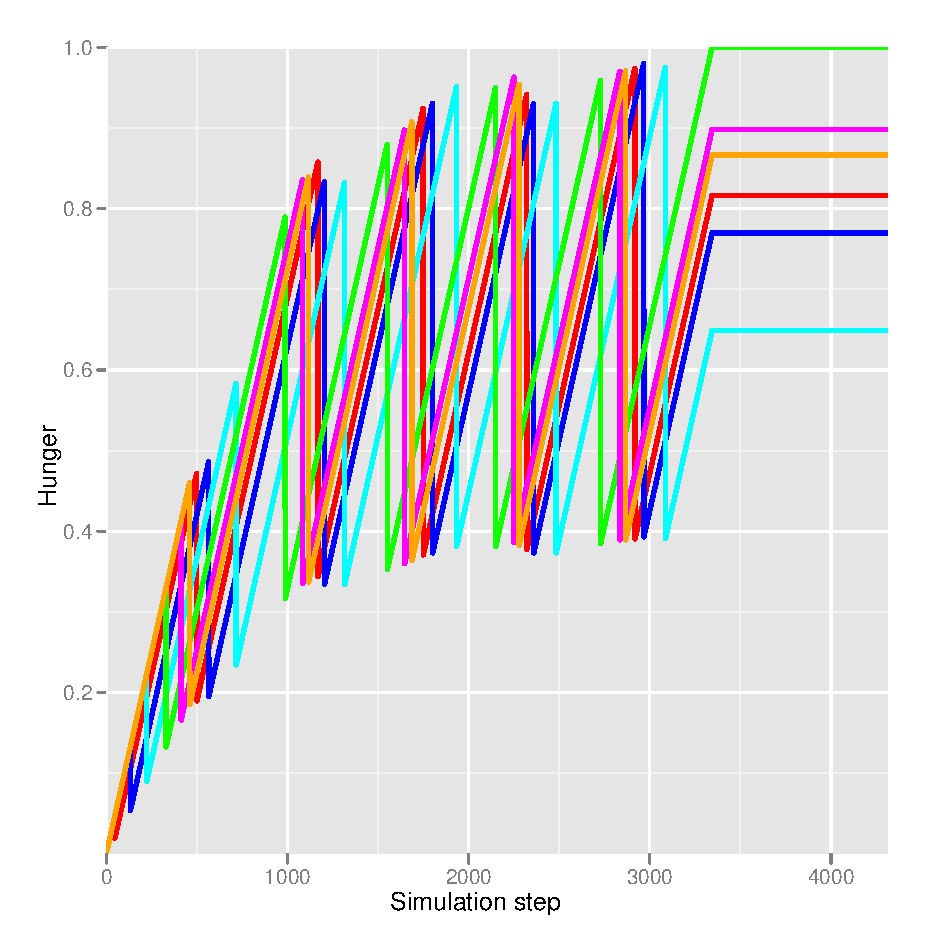
\includegraphics[scale=0.4]{diagrams/experiments/random_start.eps}    
  \caption{A beginning of life of a random agent with communication.}
  \label{experiments:random-start}
\end{figure}        

\clearpage

\subsection{PR agent}

In case of the \emph{pure reactive agents} there is not much to compare between simulation with and without the communication, because the communication is not used since the PR agents see all the environment. So both graphs \ref{experiments:pr} and \ref{experiments:pr-silent} are the same.

\begin{center}   
  \begin{tabular}{l*{6}{c}r}
  Agent kind        & median & mean & min & max \\
  \hline  
  PR agents with communication        & 0.69 & 0.689 & 0.54 & 0.86 \\
  PR agents without communication     & 0.69 & 0.689 & 0.54 & 0.86 \\
  \end{tabular}                  
\end{center}

%[1] "pr median 0.69 mean 0.688658088456766 min 0.54 max 0.86"
%[1] "pr_silent median 0.69 mean 0.688658088456766 min 0.54 max 0.86"

\begin{figure}[h!]
  \centering       
  \subfigure{                         
    \includegraphics[scale=0.35]{diagrams/experiments/pr.eps} 
    \label{experiments:pr}  
  }
  \subfigure{
    \includegraphics[scale=0.35]{diagrams/experiments/pr_silent.eps}   
    \label{experiments:pr-silent} 
  }
  \caption{PR agent with and without communication.}
\end{figure} 

\clearpage

\subsection{GNG agent}

GNG agents need more information to be able to learn and to survive that is why I do not expect them to deal with it well. In case of a simulation without communication they might end up similarly to random agents, they should do better if they communicate.

\begin{center}   
  \begin{tabular}{l*{6}{c}r}
  Agent kind        & median & mean & min & max \\
  \hline  
  GNG agents with communication        & 0.69 & 0.683 & 0.49 & 0.83 \\
  GNG agents without communication        & 1 & 1 & 1 & 1 \\
  \end{tabular}                  
\end{center}

%[1] "gng median 0.69 mean 0.683386947145215 min 0.49 max 0.83"
%[1] "gng_silent median 1 mean 1 min 1 max 1"

\begin{figure}[h!]
  \centering      
  \subfigure{                          
    \includegraphics[scale=0.35]{diagrams/experiments/gng.eps}     
    \label{experiments:gng}        
  }      
  \subfigure{                                        
    \includegraphics[scale=0.35]{diagrams/experiments/gng_silent.eps}    
    \label{experiments:gng-silent}
  }
  \caption{GNG agent with and without communication.}
\end{figure} 

\clearpage

\subsection{Grid agent}            

I assumed they will do simirarly like GNG agent, i.e. they fail to survive without communication, which assumption ended up to be wrong. Grid agents are able to learn quickly the environment just by moving around randomly and there is the chance that a couple of them survive.

I have run 20 simulations with grid agents to verify the probability of grid agent's learning the environment. As in the standard experiments there were 12 agents and the following values shows the result of the tests:

%8,8,1,9,7,6,8,1,12,3,5,3,4,2,2,4,7,5,6,12

\begin{center}   
  \emph{mean}=5.56, \emph{median}=5.5, \emph{min}=1, \emph{max}=12                 
\end{center}

\begin{center}   
  \begin{tabular}{l*{6}{c}r}
  Agent kind        & median & mean & min & max \\
  \hline  
  Grid agents with communication        & 0.81 & 0.826 & 0.54 & 1 \\
  Grid agents without communication        & 0.65 & 0.771 & 0.44 & 1 \\
  \end{tabular}                  
\end{center}


%[1] "grid median 0.81 mean 0.826481608655317 min 0.54 max 1"
%[1] "grid_silent median 0.65 mean 0.771415766075108 min 0.44 max 1"

\begin{figure}[h!]
  \centering        
  \subfigure{                        
    \includegraphics[scale=0.35]{diagrams/experiments/grid.eps}   
  }
  \subfigure{                                          
    \includegraphics[scale=0.35]{diagrams/experiments/grid_silent.eps}   
  }                                
  \caption{Grid agent with and without communication.}           
  \label{experiments:gng}  
\end{figure} 

\clearpage

\section{Mixed environment}
                        
Second part of the experiments are about environment where different kinds of agents are trying to fulfill their needs. I will observer whether some kind of agents prosper from a presence of other agents or if they are not that successful as they were in a homogeneous environment in previous experiments.
                                                                                
\subsection{GNG+Grid+PR+Random agents}

First I will start with combination of all kinds of agents, whereby since there are those PR agents the others have an advantage of the perfect source of information.  

Results of a simulation with communication follow:
         
\begin{center}   
  \begin{tabular}{l*{6}{c}r}
  Agent kind        & median & mean & min & max \\
  \hline
  GNG agents        & 0.7 & 0.699 & 0.57 & 0.86  \\
  Grid agents       & 0.7 & 0.697 & 0.54 & 0.83  \\   
  PR agents         & 0.69 & 0.689 & 0.55 & 0.81 \\  
  Random agents     & 0.7 & 0.704 & 0.57 & 0.87  \\
  All agents        & 0.7 & 0.698 & 0.54 & 0.87  \\ 
  \end{tabular}                  
\end{center}
       
Results of a simulation without communication follow:
              
\begin{center}
  \begin{tabular}{l*{6}{c}r}
  Agent kind        & median & mean & min & max \\
  \hline
  GNG agents        & 1 & 1 & 1 & 1  \\
  Grid agents       & 0.61 & 0.721 & 0.47 & 1  \\   
  PR agents         & 0.58 & 0.576 & 0.44 & 0.68 \\  
  Random agents     & 1 & 1 & 1 & 1  \\
  All agents        & 1 & 0.824 & 0.44 & 1  \\ 
  \end{tabular}                    
\end{center} 

%[1] "gng-grid-pr-random gng median 0.7 mean 0.698904096385542 min 0.57 max 0.86"
%[1] "gng-grid-pr-random grid median 0.7 mean 0.697301204819277 min 0.54 max 0.83"
%[1] "gng-grid-pr-random pr median 0.69 mean 0.68933734939759 min 0.55 max 0.81"
%[1] "gng-grid-pr-random random median 0.7 mean 0.704657124957833 min 0.57 max 0.87" 
%[1] "gng-grid-pr-random all median 0.7 mean 0.697550029517717 min 0.54 max 0.87"

%[1] "gng-grid-pr-random_silent gng median 1 mean 1 min 1 max 1"
%[1] "gng-grid-pr-random_silent grid median 0.61 mean 0.721167710843373 min 0.47 max 1"
%[1] "gng-grid-pr-random_silent pr median 0.58 mean 0.575706712929497 min 0.44 max 0.68"
%[1] "gng-grid-pr-random_silent random median 1 mean 1 min 1 max 1"  
%[1] "gng-grid-pr-random_silent all median 1 mean 0.824215611860098 min 0.44 max 1"

\begin{figure}[h!]
  \centering        
  \subfigure{                        
    \includegraphics[scale=0.35]{diagrams/experiments/gng-grid-pr-random.eps}    
    \label{experiments:gng-grid-pr-random}
  }     
  \subfigure{
    \includegraphics[scale=0.35]{diagrams/experiments/gng-grid-pr-random_silent.eps}    
    \label{experiments:gng-grid-pr-random-silent}
  }                                                       
  \caption{GNG, grid, PR and random agents together. Owing to PR agents and the communication they all do well.}
\end{figure}
       
\clearpage
                                
\subsection{GNG+Grid+Random agents}

In this experiment I have omitted pure reactive agents and thus left others on their own. For better comparision I have added the difference between values in the current experiment and the previous one (GNG+Grid+PR+Random). I used red colour for a decrease and green colour for an increase, although it is an improvement if they values are lower.         
             
\begin{center}
  \begin{tabular}{l*{6}{c}r}
  Agent kind        & median & mean & min & max \\
  \hline
  GNG agents        & 0.69                  & 0.691                   & 0.52                  & 0.86  \\
                    & \color{red}{-0.01}  & \color{red}{-0.008}   & \color{red}{-0.05}  &       \\
  Grid agents       & 0.7                   & 0.700                   & 0.55                  & 0.87   \\   
                    &                       & \color{green}{+0.003} & \color{green}{+0.01}& \color{green}{+0.04} \\
  Random agents     & 0.7                   & 0.702                   & 0.55                  & 0.85   \\
                    &                       & \color{red}{-0.002}   & \color{red}{-0.02}  & \color{red}{-0.02}  \\
  All agents        & 0.7                   & 0.698                   & 0.52                  & 0.87  \\
                    &                       &                         & \color{red}{-0.02}  &       \\
  \end{tabular}                                
\end{center}

\begin{center} 
  \begin{tabular}{l*{6}{c}r}
  Agent kind        & median & mean & min & max \\
  \hline
  GNG agents        & 1 & 1 & 1 & 1  \\
                    &   \\
  Grid agents       & 1                     & 0.747                 & 0.39                & 1  \\  
                    & \color{green}{+0.39}  & \color{green}{0.026}  & \color{red}{-0.08}  \\
  Random agents     & 1 & 1 & 1 & 1  \\         
                    & \\
  All agents        & 1 & 0.916                 & 0.39 & 1  \\  
                    &   & \color{green}{+0.092}  & \color{red}{-0.05} \\
  \end{tabular}                                        
\end{center}

%[1] "gng-grid-random gng median 0.69 mean 0.69148588571222 min 0.52 max 0.86"
%[1] "gng-grid-random grid median 0.7 mean 0.699864820905772 min 0.55 max 0.87"
%[1] "gng-grid-random random median 0.7 mean 0.702296598836159 min 0.55 max 0.85"  
%[1] "gng-grid-random all median 0.7 mean 0.697882435151384 min 0.52 max 0.87"

%[1] "gng-grid-random_silent gng median 1 mean 1 min 1 max 1"
%[1] "gng-grid-random_silent grid median 1 mean 0.747429428561102 min 0.39 max 1"
%[1] "gng-grid-random_silent random median 1 mean 1 min 1 max 1"           
%[1] "gng-grid-random_silent all median 1 mean 0.915809809520367 min 0.39 max 1"

\begin{figure}[h!]
  \centering      
  \subfigure{                          
    \includegraphics[scale=0.35]{diagrams/experiments/gng-grid-random.eps}    
    \label{experiments:gng-grid-random}
  }                                                                              
  \subfigure{                                                  
    \includegraphics[scale=0.35]{diagrams/experiments/gng-grid-random_silent.eps}      
    \label{experiments:gng-grid-random-silent}                                     
  }
  \caption{GNG, grid, PR agents together with and without the communication.}
\end{figure} 
              
\clearpage
                                       
\subsection{GNG+Grid agents}

In this experiment I have observed a simulation with just memory agents in it. Again you can see highlighted differences between new values from this experiment and the values from the previous one (GNG+Grid+Random).

\begin{center} 
  \begin{tabular}{l*{6}{c}r}
  Agent kind        & median & mean & min & max \\
  \hline
  GNG agents        & 0.72                  & 0.715                 & 0.5                 & 0.89  \\  
                    & \color{green}{+0.03}  & \color{green}{+0.024} & \color{red}{-0.02}  & \color{green}{+0.03} \\
  Grid agents       & 0.72                  & 0.721                 & 0.57                & 0.89  \\  
                    & \color{green}{+0.02}  & \color{green}{+0.021} & \color{green}{+0.02}& \color{red}{+0.02}   \\
  All agents        & 0.72                  & 0.718                 & 0.5                 & 0.89  \\
                    & \color{green}{+0.02}  & \color{green}{+0.020}  & \color{red}{-0.02}  & \color{green}{+0.02} 
  \end{tabular}                       
\end{center}

\begin{center}
  \begin{tabular}{l*{6}{c}r}
  Agent kind        & median & mean & min & max \\
  \hline
  GNG agents        & 1 & 1 & 1 & 1  \\   
                    & \\
  Grid agents       & 1 & 0.755                 & 0.4 & 1  \\  
                    &   & \color{green}{+0.008} & \color{green}{+0.01}  \\
  All agents        & 1 & 0.877               & 0.4 & 1  \\
                    &   & \color{red}{-0.039} & \color{green}{0.01} \\
  \end{tabular}                                 
\end{center}

%[1] "gng-grid gng median 0.72 mean 0.714870602409639 min 0.5 max 0.89"
%[1] "gng-grid grid median 0.72 mean 0.721010337100311 min 0.57 max 0.89" 
%[1] "gng-grid all median 0.72 mean 0.717940506740883 min 0.5 max 0.89"

%[1] "gng-grid_silent gng median 1 mean 1 min 1 max 1"
%[1] "gng-grid_silent grid median 1 mean 0.755093371244066 min 0.4 max 1" 
%[1] "gng-grid_silent all median 1 mean 0.877545210298671 min 0.4 max 1"

\begin{figure}[h!]
  \centering          
  \subfigure{                      
    \includegraphics[scale=0.35]{diagrams/experiments/gng-grid.eps}
    \label{experiments:gng-grid}
  }
  \subfigure{                                              
    \includegraphics[scale=0.35]{diagrams/experiments/gng-grid_silent.eps} 
    \label{experiments:gng-grid-silent}  
  }
  \caption{GNG and grid agents together.}
\end{figure}

\chapter{Discussion}

In previous chapter you have seen experimental runs of the simulation where I have compared the level of overall hunger of agents throughout the simulation's steps. Now I am going to sum up those results and discuss possible outcomes.

%[single-kind environment]

Simulation settings (size of the environment, number and distribution of resources) allowed random agents to survive few steps when they could communicate with each others. Thereby the communication was strong tool for agents how to improve their results.

The communication was not always an improvement as you can see in \ref{experiments:gng} where the grid agents were less efficient when they were allowed to share information about the environment. The communication brings more income information and thus increases the ration between positive and negative variables (see \ref{sec:grid}) and disorients agents. Owing to communicatio it is hard to decide which of gng and grid agent was better.

As I have already clarified the grid agent has perfect results without using communication as soon as he survives first thousand steps. On the other hand, he obviously fails to use communication as an improving factor. That is something where the gng agents win.

%[mixed environment]

Second part of experiments is about comparing simulation with more kinds of agents at once. Thereby I could observe how they compete against each others. So I have observed GNG+Grid+PR+Random, GNG+Grid+Random and GNG+Grid. Apart experiments with communication, I have also run simulation whereby the agents were not able to communication, although in such conditions the result could not be different from single-kind setups.

Since there are pure reactive agents in the first experiment (GNG+Grid+PR+Random) the agents have a perfect source of information and thus easily succeeded. Having omitted PR agents I could have observed that gng agents have bettered and, on the other hand, the grid agent become worse. Furthermore, when you look at results of GNG+Grid simulation where the random agents are missing, you can see that both grid and gng agents become worse, although the random agents should be much helpfull. 

What is different between random agents and memory agents is the random agent answers only correct positions, when he is asked, and the memory agent usually answers using his believes.

%[problems]

There were minor problems I had to deal with, summary of which follows.

First I had to setup variables for the GNG algorithm. What I have learnt from that is the algorithm is expected to slowly converge to the learnt topology. On the other hand, I have used it for unncertain dynamicly changing data which were mostly based on other agents' believes. That is probably why much simpler memory structure used for grid agents has better results.

...

 



\chapter{Conclusions}

I have created a multi-agent simulation with four different kinds of agents each of which differs in their approach to fulfill their needs. What they had to succeed in was they were put inside a two dimensional environment whereby they had to learn positions of six food resource so as to be able to survive. They were pure reactive agent, random agent, GNG agent and grid agent. Latter two had a memory to learn those positions. GNG agent used implemantion of growing neural gas, an unsupervised neural network, and grid agent used data structure inspired by \cite{Brom:placeandobjects}.

My goal was to compare those agents how good they were. These result are presented in previous chapter. [Summary of the results.] There were minor problems I had to deal with summary of which follows.

First I had to setup variables for the GNG algorithm. What I have learnt from that is the algorithm is expected to slowly converge to the learnt topology. On the other hand, I have used it for unncertain dynamicly changing data which were mostly based on other agents' believes. That is probably why much simpler memory structure used for grid agents has better results.

 


%%% Seznam literatury
%%%
%%% Literatura se řadí abecedně. Úvádí se pouze literatura, na kterou se v textu odkazuje.
%%% Při odkazu na knihu se vždy uvádějí čísla stránek.

\addcontentsline{toc}{chapter}{Bibliography}
\bibliographystyle{plain}
\bibliography{bc_thesis}
  
\end{document}
